\documentclass[12pt]{article}
\usepackage[utf8]{inputenc}
\usepackage{graphicx,geometry,tikz,pgfplots,pgfplotstable,listings}
\usetikzlibrary{shapes,automata,fit}
\geometry{a4paper,total={500pt,750pt}}
\DeclareGraphicsExtensions{.pdf,.png,.jpg}
\setcounter{secnumdepth}{0}
\linespread{1.0}
\pagestyle{empty}

\tikzset{nurse/.style={circle, draw, fill=blue!20, minimum size=0.64cm}}
\tikzset{queue/.style={diamond, draw, fill=yellow!20, minimum size=0.28cm}}
\tikzset{bed/.style={rectangle, draw, fill=red!20, minimum size=0.64cm}}
\tikzset{home/.style={regular polygon, regular polygon sides=3, draw, fill=green!20, minimum size=0.36cm}}


\definecolor{codegreen}{rgb}{0,0.6,0}
\definecolor{codegray}{rgb}{0.5,0.5,0.5}
\definecolor{codepurple}{rgb}{0.58,0,0.82}
\definecolor{backcolour}{rgb}{0.95,0.95,0.92}

\lstdefinestyle{mystyle}{
    backgroundcolor=\color{backcolour},   
    commentstyle=\color{codegreen},
    keywordstyle=\color{magenta},
    numberstyle=\tiny\color{codegray},
    stringstyle=\color{codepurple},
    basicstyle=\ttfamily\footnotesize,
    breakatwhitespace=false,
    breaklines=true,
    captionpos=b,
    keepspaces=true,                
    numbersep=5pt,
    showspaces=false,
    showstringspaces=false,
    showtabs=false,
    tabsize=2
}

\lstset{style=mystyle}


\begin{document}
\thispagestyle{empty}

\begin{center}
\begin{tabular}{|*{4}{c|}}
\hline
event: init & \multicolumn{3}{c|}{time: 0.0} \\
\hline
system & \multicolumn{3}{c|}{
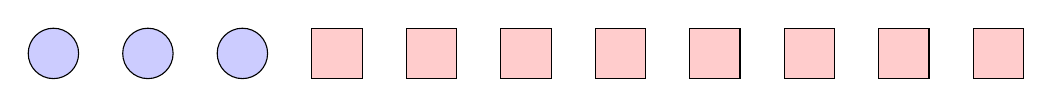
\begin{tikzpicture}[baseline=(current bounding box.north)]
\node[nurse] at (1.2, 0) {};\node[nurse] at (2.4, 0) {};\node[nurse] at (3.5999999999999996, 0) {};\node[bed] at (4.8, 0) {};\node[bed] at (6.0, 0) {};\node[bed] at (7.199999999999999, 0) {};\node[bed] at (8.4, 0) {};\node[bed] at (9.6, 0) {};\node[bed] at (10.799999999999999, 0) {};\node[bed] at (12.0, 0) {};\node[bed] at (13.2, 0) {};
\end{tikzpicture}
} \\
\hline
calendar & \multicolumn{3}{c|}{(A0, 2.0008282460714533)} \\
\hline
healed & B(t) & N(t) & Q(t) \\
0 & 0/8 & 0/3 & 0 \\
\hline
\multicolumn{4}{|c|}{
\begin{tikzpicture}[baseline=(current bounding box.north)]
\begin{axis}[
    xlabel={time},
    ylabel={B(t)},
    xmin=-0.5, xmax=14.5,
    ymin=-0.5, ymax=8.5,
    ytick={0, 1, 2, 3, 4, 5, 6, 7, 8},
    legend pos=north east,
    scale only axis, width=14cm, height=6cm
]
\addplot [color=blue, mark=square*, const plot]
coordinates {
    (0.0, 0)
};
\end{axis}
\end{tikzpicture}
} \\
\hline
\multicolumn{4}{|c|}{
\begin{tikzpicture}[baseline=(current bounding box.north)]
\begin{axis}[
    xlabel={time},
    ylabel={N(t)},
    xmin=-0.5, xmax=14.5,
    ymin=-0.5, ymax=3.5,
    ytick={0, 1, 2, 3},
    legend pos=north east,
    scale only axis, width=14cm, height=2.25cm
]
\addplot [color=blue, mark=square*, const plot]
coordinates {
    (0.0, 0)
};
\end{axis}
\end{tikzpicture}
} \\
\hline
\multicolumn{4}{|c|}{
\begin{tikzpicture}[baseline=(current bounding box.north)]
\begin{axis}[
    xlabel={time},
    ylabel={Q(t)},
    xmin=-0.5, xmax=14.5,
    ymin=-0.5, ymax=3.5,
    ytick={0, 1, 2, 3},
    legend pos=north east,
    scale only axis, width=14cm, height=2.25cm
]
\addplot [color=blue, mark=square*, const plot]
coordinates {
    (0.0, 0)
};
\end{axis}
\end{tikzpicture}
} \\
\hline
\end{tabular}
\end{center}
\newpage

\begin{center}
\begin{tabular}{|*{4}{c|}}
\hline
event: H1 & \multicolumn{3}{c|}{time: 13.750025107066259} \\
\hline
system & \multicolumn{3}{c|}{
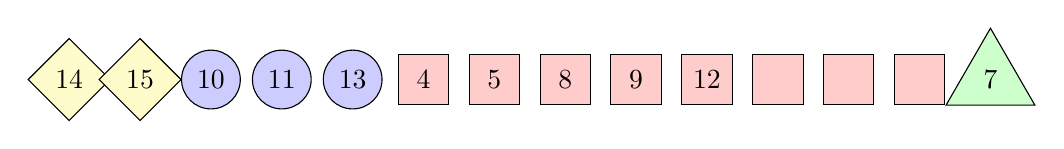
\begin{tikzpicture}[baseline=(current bounding box.north)]
\node[queue] at (0.9, 0) {14};\node[queue] at (1.8, 0) {15};\node[nurse] at (2.7, 0) {10};\node[nurse] at (3.6, 0) {11};\node[nurse] at (4.5, 0) {13};\node[bed] at (5.4, 0) {4};\node[bed] at (6.3, 0) {5};\node[bed] at (7.2, 0) {8};\node[bed] at (8.1, 0) {9};\node[bed] at (9.0, 0) {12};\node[bed] at (9.9, 0) {};\node[bed] at (10.8, 0) {};\node[bed] at (11.700000000000001, 0) {};\node[home] at (12.6, 0) {7};
\end{tikzpicture}
} \\
\hline
calendar & \multicolumn{3}{c|}{\shortstack{(A16, 14.213004146930912)\\(E13, 15.255253530032837)\\(H12, 15.297317020890079)\\(H5, 15.362798648707884)\\(E11, 17.06158742007228)\\(H8, 17.555739854857276)\\(E10, 18.834916505512616)\\(H9, 22.558569367342997)\\(H4, 24.549688453219886)\\(H7, 28.19515396011098)}} \\
\hline
healed & B(t) & N(t) & Q(t) \\
5 & 5/8 & 3/3 & 2 \\
\hline
\multicolumn{4}{|c|}{
\begin{tikzpicture}[baseline=(current bounding box.north)]
\begin{axis}[
    xlabel={time},
    ylabel={B(t)},
    xmin=-0.5, xmax=14.5,
    ymin=-0.5, ymax=8.5,
    ytick={0, 1, 2, 3, 4, 5, 6, 7, 8},
    legend pos=north east,
    scale only axis, width=14cm, height=6cm
]
\addplot [color=blue, mark=square*, const plot]
coordinates {
    (0.0, 0) (2.0008282460714533, 0) (2.4921810789076195, 0) (2.492798392969369, 0) (3.6206274040246615, 1) (3.9692166650544203, 1) (4.1496117711817595, 1) (5.38753325258501, 1) (7.376132862956432, 2) (7.657822610519585, 2) (7.891598533807141, 3) (8.032747599727156, 2) (8.393617769562074, 2) (8.911937686687331, 3) (9.107393674141067, 2) (9.397259335530556, 2) (9.436624295224057, 2) (9.680315036662922, 1) (9.730291004904126, 1) (9.749205496597863, 1) (9.795557882523216, 2) (10.032588570910459, 3) (10.30377127519566, 3) (10.753640296468985, 4) (11.429682775325166, 4) (12.368154759975976, 4) (12.712536423788938, 5) (13.357138803397095, 5) (13.374072888623424, 5) (13.481616871045256, 5) (13.542784411114406, 5) (13.562384413869966, 6) (13.750025107066259, 5)
};
\end{axis}
\end{tikzpicture}
} \\
\hline
\multicolumn{4}{|c|}{
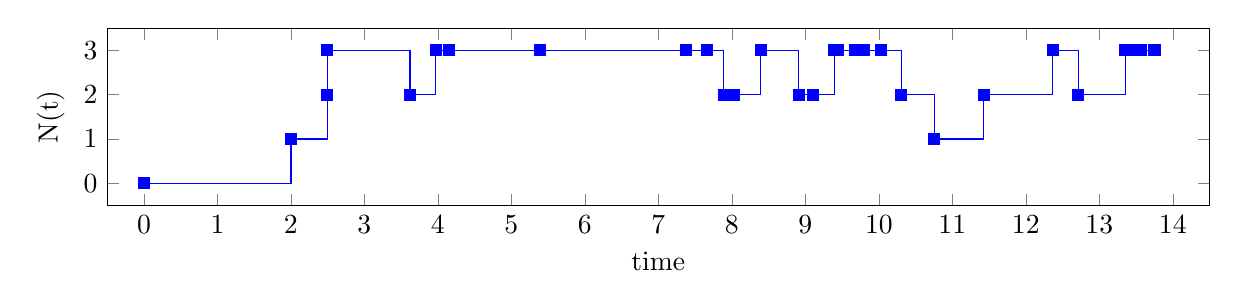
\begin{tikzpicture}[baseline=(current bounding box.north)]
\begin{axis}[
    xlabel={time},
    ylabel={N(t)},
    xmin=-0.5, xmax=14.5,
    ymin=-0.5, ymax=3.5,
    ytick={0, 1, 2, 3},
    legend pos=north east,
    scale only axis, width=14cm, height=2.25cm
]
\addplot [color=blue, mark=square*, const plot]
coordinates {
    (0.0, 0) (2.0008282460714533, 1) (2.4921810789076195, 2) (2.492798392969369, 3) (3.6206274040246615, 2) (3.9692166650544203, 3) (4.1496117711817595, 3) (5.38753325258501, 3) (7.376132862956432, 3) (7.657822610519585, 3) (7.891598533807141, 2) (8.032747599727156, 2) (8.393617769562074, 3) (8.911937686687331, 2) (9.107393674141067, 2) (9.397259335530556, 3) (9.436624295224057, 3) (9.680315036662922, 3) (9.730291004904126, 3) (9.749205496597863, 3) (9.795557882523216, 3) (10.032588570910459, 3) (10.30377127519566, 2) (10.753640296468985, 1) (11.429682775325166, 2) (12.368154759975976, 3) (12.712536423788938, 2) (13.357138803397095, 3) (13.374072888623424, 3) (13.481616871045256, 3) (13.542784411114406, 3) (13.562384413869966, 3) (13.750025107066259, 3)
};
\end{axis}
\end{tikzpicture}
} \\
\hline
\multicolumn{4}{|c|}{
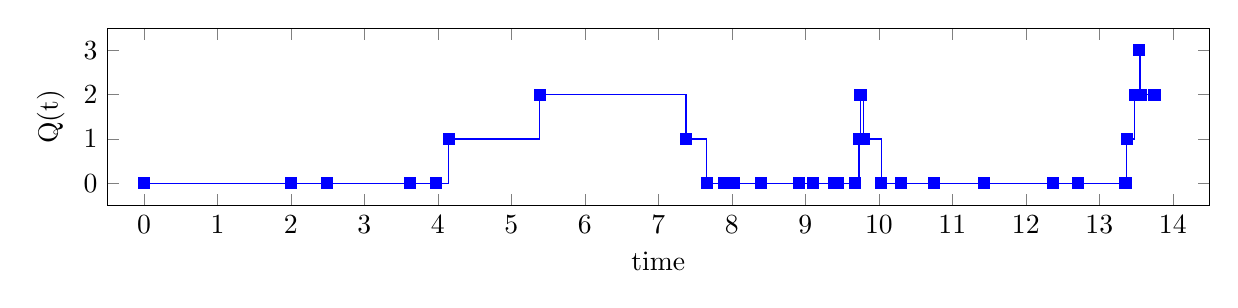
\begin{tikzpicture}[baseline=(current bounding box.north)]
\begin{axis}[
    xlabel={time},
    ylabel={Q(t)},
    xmin=-0.5, xmax=14.5,
    ymin=-0.5, ymax=3.5,
    ytick={0, 1, 2, 3},
    legend pos=north east,
    scale only axis, width=14cm, height=2.25cm
]
\addplot [color=blue, mark=square*, const plot]
coordinates {
    (0.0, 0) (2.0008282460714533, 0) (2.4921810789076195, 0) (2.492798392969369, 0) (3.6206274040246615, 0) (3.9692166650544203, 0) (4.1496117711817595, 1) (5.38753325258501, 2) (7.376132862956432, 1) (7.657822610519585, 0) (7.891598533807141, 0) (8.032747599727156, 0) (8.393617769562074, 0) (8.911937686687331, 0) (9.107393674141067, 0) (9.397259335530556, 0) (9.436624295224057, 0) (9.680315036662922, 0) (9.730291004904126, 1) (9.749205496597863, 2) (9.795557882523216, 1) (10.032588570910459, 0) (10.30377127519566, 0) (10.753640296468985, 0) (11.429682775325166, 0) (12.368154759975976, 0) (12.712536423788938, 0) (13.357138803397095, 0) (13.374072888623424, 1) (13.481616871045256, 2) (13.542784411114406, 3) (13.562384413869966, 2) (13.750025107066259, 2)
};
\end{axis}
\end{tikzpicture}
} \\
\hline
\end{tabular}
\end{center}

\end{document}
